\documentclass[conference]{IEEEtran}
% \IEEEoverridecommandlockouts
% The preceding line is only needed to identify funding in the first footnote. If that is unneeded, please comment it out.
%Template version as of 6/27/2024

\usepackage[noadjust]{cite}
\usepackage{amsmath,amssymb,amsfonts}
\usepackage{algorithmic}
\usepackage{graphicx}
\usepackage[hidelinks]{hyperref}
\usepackage{textcomp}
\usepackage{xcolor}

\usepackage[brazil]{babel}
\addto\captionsbrazil{%
  \renewcommand\abstractname{Resumo }%
  \renewcommand\IEEEkeywordsname{Palavras-chave }%
}
\def\BibTeX{{\rm B\kern-.05em{\sc i\kern-.025em b}\kern-.08em
    T\kern-.1667em\lower.7ex\hbox{E}\kern-.125emX}}
\begin{document}

\hypersetup{
    colorlinks=false,
    pdftitle={Sintetizando episódios de treino via abstração de jogos em aprendizado por reforço},
    pdfpagemode=FullScreen,
    }

\title{Sintetizando episódios de treino via abstração de jogos em aprendizado por reforço}

\author{\IEEEauthorblockN{Marcelo Augusto Salomão Ganem}
\IEEEauthorblockA{\textit{Departamento de Ciência da Computação (UFMG)} \\
Belo Horizonte, Minas Gerais \\
marceloganem@dcc.ufmg.br}
}

\maketitle

\begin{abstract}
    \space Este trabalho propõe uma metodologia para sintetizar episódios de treino em aprendizado por reforço a partir de abstrações de jogos baseadas na sintaxe Machinations, traduzindo-as formalmente em Processos de Decisão de Markov (MDPs). Inicialmente, definimos nós, gatilhos, conexões de recursos e modificadores como componentes de um diagrama cuja ativação e transferência de recursos geram a dinâmica de transição de estados observáveis e parcialmente observáveis. Em seguida, modelamos dois jogos clássicos — Blackjack e Monopoly — sob essa representação simplificada, visando avaliar a viabilidade do método como pré-otimização de políticas. Experimentos de aprendizado por reforço foram executados para a modelagem de Monopoly: Deep Q-Networks (DQNs) não convergiram, enquanto agentes treinados com Proximal Policy Optimization (PPO), utilizando Generalized Advantage Estimation e função de objetivo com clipping, superaram a linha de base aleatória (sobrevivência média de 17,7 versus 14 turnos em um ambiente altamente estocástico) porém ainda apresentaram desempenho limitado em razão da alta estocasticidade e recompensas esparsas. Discutimos, por fim, as implicações para curriculum learning e as perspectivas de transferência do conhecimento adquirido no ambiente abstrato para implementações reais de jogos.
\end{abstract}

\begin{IEEEkeywords}
    \space reinforcement learning, game modeling, board games, curriculum learning
\end{IEEEkeywords}

\section{Introdução}
\label{intro}
Um desafio central abordado pela literatura de aprendizado por reforço há mais de duas décadas é a combinação de planejamento e aprendizado de maneira a minimizar a necessidade de intervenções humanas e maximizar a generalização dos comportamentos obtidos. Dentre as formas mais tradicionais de introduzir estrutura a partir de conhecimento especializado em soluções de aprendizado por reforço está a construção de \textit{features} que sejam uma abstração suficientemente representativa do ambiente apresentado ao agente. 

Especificamente no domínio de jogos (virtuais e de tabuleiro), um obstáculo frequentemente encontrado é a complexidade de regras e relações que precisam ser implicitamente compreendidas pelo agente. Mesmo que triviais para humanos, a combinação de um conjunto de regras suficientemente ortogonais entre si é capaz de produzir dinâmicas e estados com padrões ruidosos que, quando não explicados por um conjunto de regras explícitas, demandam aproximadores de funções complexos e treinamento extensivo para serem identificados.

Joris Dormans\cite{machinations} investiga a produção do chamado comportamento emergente em jogos, propondo uma sintaxe relativamente simples capaz de evidenciar os recursos e entidades centrais em um jogo, bem como as relações entre essas entidades. Assim, de acordo com Dormans, é possível rapidamente identificar ciclos de retroalimentação que ditam a economia geral de um jogo.

Os diagramas construídos pela sintaxe proposta, enquanto conceitualmente sob domínio público, não estão mais publicamente disponíveis para teste e simulação -- a empresa Machinations SARL\footnote{\url{https://machinations.io/about}} atualmente oferece esse serviço de maneira privada a empresas de desenvolvimento e design de jogos. Ao longo da última década, publicações pontuais exploraram a aplicabilidade das proposições de Dormans no contexto de Inteligência Artificial.\footnote{\url{https://machinations.io/resources/academic-research-publications}}


\section{Objetivos}
\label{goals}

O presente trabalho visa, portanto, construir uma representação simplificada e formalizada de diagramas  Machinations para representar um conjunto amplo de jogos compreendidos pela combinação dos elementos e conexões disponíveis. 

A partir disso, investigamos a aplicabilidade dessas representações simplificadas no treino de agentes de aprendizado por reforço como uma pré-otimização com respeito à verdadeira política ótima -- dentre as múltiplas formas de utilizar a riqueza semântica e estrutural dessas representações na construção de modelos de IA.

\section{Trabalhos Relacionados}
A hipótese aqui investigada se sustenta centralmente, além de em conceitos da literatura geral de aprendizado por reforço, em trabalhos que propõem, viabilizam e justificam a utilização de representações abstrativas e simplificadas para pelo menos parte do aprendizado.

\subsection{Engineering Emergence}
\label{references:machinations}
O elemento central do trabalho "\textit{Engineering Emergence: Applied Theory for Game Design}"\cite{machinations} é a definição de uma gramática de elementos para a composição de uma estrutura semelhante a um grafo cuja premissa é representar o estado da economia interna de um jogo.
\begin{figure}[h!]
    \centering
    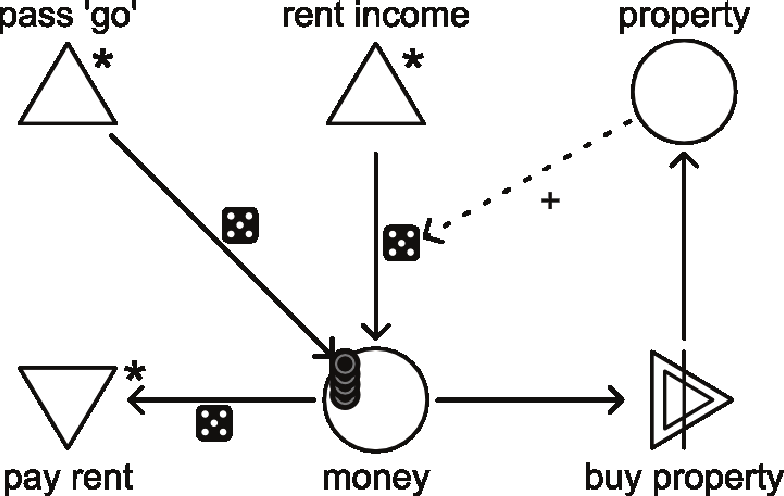
\includegraphics[width=0.9\linewidth]{figures/monopoly.png}
    \caption{Representação do jogo \textit{Monopoly} sob a sintaxe \textit{Machinations}.}.
    \label{fig:monopoly}
\end{figure}

O autor define essa economia interna como a alocação dos recursos (representados na Figura \ref{fig:monopoly} como fichas em cima de cada nó) entre os nós. O estado dessa economia é alterado a partir do andamento discreto do tempo e ações do jogador ou de quaisquer agentes presentes no sistema. O caráter dessas transições, i.e., o estado atingido em seguida, é ditado pelas arestas do grafo, que indicam transferência regular, condicional ou probabilística de recursos.

Como mencionado na Seção \ref{goals}, visamos construir uma versão formal e simplificada dos elementos e regras propostas por Dormans. A Seção \ref{modeling} se dedica à transcrição das definições originais para o contexto de um Processo de Decisão de Markov (MDP) adequado para aprendizado por reforço.

\subsection{Curriculum Learning}
A premissa de que um agente é capaz de aprender uma representação útil da política ótima no problema final a partir de uma versão simplificada de um problema é firmada no conceito de curriculum learning. Especificamente, Bengio et al.\cite{curriculum} formalizam a intuição de que apresentar tarefas de dificuldade crescente em ordem durante o treinamento de um agente é mais efetivo do que apresentar o problema completo.

Nesse sentido, o treinamento de um agente de aprendizado por reforço em um diagrama Machinations suficientemente representativo pode ser visto como uma otimização não-refinada com respeito ao problema original. Naturalmente, essa premissa é sensível à qualidade da representação abstrata, i.e., o quanto a dinâmica do problema original apresenta um comportamento coerente em comparação à dinâmica simplificada.

\subsection{Relational Reinforcement Learning}
Tadepalli et al. \cite{rrl} investigaram há mais de duas décadas a relevância da ideia de representações relacionalmente estruturadas no contexto de aprendizado por reforço. Especificamente, os autores observam que diversas das técnicas de aprendizado por reforço apresentadas à época -- de fato, grande parte das técnicas de aprendizado por reforço até hoje -- introduziam informações semanticamente relacionais sobre o problema de formas diferentes.

A introdução de diagramas Machinations como um ambiente de treino pode ser vista como mais um caso da observação feita: primeiro, o agente é exposto a um ambiente que compreende estritamente os elementos centrais da economia de um jogo e que se comporta conforme as relações mais significativas entre eles. Observando o estado do diagrama, de dimensionalidade tipicamente inferior a representações reais (sobretudo de jogos virtuais), o aprendizado necessário é essencialmente da relação numérica entre as variáveis observadas -- e quais delas estão correlacionadas a recompensas positivas e negativas.

\subsection{A modeling environment for reinforcement learning in games}
"A modeling environment for reinforcement learning in games" coincide com o presente trabalho na busca por uma solução genérica e explicável para a produção consistente e controlável de comportamentos artificialmente inteligentes. Gomes et al.\cite{modeling-rl-games} declaram um objetivo muito semelhante:
\begin{quote}
    Thus, AI4U was specifically refined to the preparation of reinforcement learning experiments in games. In general, the high-level goals of this environment are: to enable the reproducibility of methods and results; \textbf{to simplify the way of designing reinforcement learning algorithms in games;} and to enhance the readability of RL agents.
\end{quote}

A solução apresentada pelos autores se centraliza na definição de uma ontologia de elementos e comportamentos compatíveis com definições comuns em engines de jogos, tal que desenvolvedores são capazes de especificar elementos das interações e regras desejadas para reforçar comportamentos em personagens não jogáveis. Observamos, assim, uma evidência da eficácia da introdução de uma simplificação relacional estruturada como linguagem única para a produção de uma solução em aprendizado por reforço.

\section{Metodologia}

O problema proposto é abordado primeiro pela modelagem dos elementos e regras universais a todas as simulações simplificadas sob o prisma de um MDP. Então, modelamos os jogos Blackjack e Monopoly para verificar a capacidade do novo conjunto de definições básicas. Por fim, aplicamos Proximal Policy Optimization\cite{ppo} ao cenário simulado do Monopoly para verificar a capacidade de convergência do agente para a política ótima no cenário proposto.

As dificuldades enfrentadas na parte de aprendizado, elaboradas na Seção \ref{results}, dificultam a extensão dos agentes treinados nas simulações para o problema real. Dedicamos este estudo, portanto, à investigação das propriedades dos diagramas implementados no contexto de aprendizado por reforço, bem como dos obstáculos encontrados.

\subsection{Modelagem}
\label{modeling}
Definimos um diagrama como um conjunto $(V, E)$ de nós e conexões que possuem tipos, propriedades e estados específicos. Vale ressaltar que, formalmente, é incorreto classificar esse diagrama como um grafo dada a existência de arestas $e:(v\rightarrow e')$.

\subsubsection{Nós}
Seguindo a definição central da sintaxe Machinations, nós $v \in V$ possuem um estado correspondente $X_{v,r,t} \in \mathbb{R}$ que indica a quantidade de recursos do tipo $r$ no nó $v$ no instante $t$. Nós têm um de quatro modos de ativação:\footnote{Condensando a separação entre nós e gates originalmente definida por Dormans} passivo, automático, interativo ou não-determinístico. Inicialmente, nós podem ter atribuídos a si uma distribuição de valores a amostrar para cada tipo de recurso. Nesse caso, sempre que o nó $v$ é ativado, o estado $X_{v,r,t}$ é redefinido como uma amostra aleatória dentre os valores dessa distribuição -- que pode opcionalmente se esgotar ou ser infinita.

\subsubsection{Ativação}
A ativação de nós é ditada pelo seu modo de ativação e pelos gatilhos $e \in E^G \subset E$ e ativadores $e \in E^A \subset E$ a eles direcionados. Especificamente, nós passivos só são ativados pela ação de gatilhos; nós automáticos são ativados a todo instante; nós interativos são ativados por ação do agente; nós não-determinísticos sobrescrevem seu estado por uma amostra aleatória a todo instante, mas não se ativam. Por fim, nenhum nó ou gatilho pode ser ativado caso o predicado $P_e$ de um ativador $e$ direcionado a ele seja falso.

\subsubsection{Condições}
No contexto destas simulações, predicados representam condições matemáticas simples em função do nó de origem de uma aresta que podem bloquear com precedência absoluta a ativação do alvo (ou da própria conexão, no caso de gatilhos).

Gatilhos podem ser passivos, ativando-se somente a partir da ativação do nó de onde saem, ou automáticos, ativando-se sempre que seu predicado $P_e$ estiver ativo. Um gatilho passivo que possui um predicado se ativa somente quando seu predicado está ativo.

\subsubsection{Transferência de recursos}
A ativação de um nó têm, portanto, duas consequências: a ativação dos gatilhos e de todas as conexões de recursos saindo de si. Uma conexão de recurso $e \in E^R \subset E$ transfere $T_{e,t}$ recursos do tipo $\tau_e \in R$ do seu nó de origem para o nó alvo quando ativada -- seguindo as mesmas regras que nós seguem para gatilhos e ativadores. Aqui, $R$ representa o conjunto de todos os tipos de recursos existentes no diagrama.

Modificadores são os elementos responsáveis pela construção de padrões assintóticos na economia dos recursos entre os nós. Um modificador $e \in E^M$ tem como alvo um nó ou conexão de recurso que, a todo instante $t$, tem a taxa $\dot{T}_e$  multiplicada pelo estado $X_{v,\tau_{\text{(SRC)}e},t}$ do nó de origem adicionada ao seu estado $X_{v,\tau_{\text{(DST)}e},t}$, no caso de um alvo $v \in V$, ou simplesmente $T_{e'}$, no caso de um alvo $e' \in E^R$. Vale notar que a taxa de modificadores é estática e, portanto, não subscrita pelo indicador de tempo.

\subsection{Ações}

Definimos as ações do MDP construído como o conjunto potência dos nós interativos. Essa definição é consistente com as regras para nós interativos propostas por Dormans: um agente é capaz de tomar entre cada uma e nenhuma das ações disponibilizadas pelos nós interativos do diagrama. Sendo $V^I \subset V$ o conjunto dos nós interativos, temos:

$$
\mathbf{A} = \mathcal{P}(V^I)
$$

\subsection{Estados}

O estado é composto por quaisquer elementos do diagrama que mudem ao longo do tempo. Observa-se, evidentemente, que essa representação é insuficiente para treinar agentes capazes de lidar com diferentes diagramas. Limitamo-nos aqui ao treino de um agente que busca aprender uma representação fixa de um único jogo.

Ainda, nem todos os aspectos da economia de um jogo são visíveis ou relevantes para o aprendizado. Temos, na verdade, um MDP parcialmente observável -- para isso, definimos subconjuntos $X^O$ e $T^O$ correspondentes aos nós e conexões de recursos observáveis tal que um estado $S_t \in \mathbf{S}$ tem a forma:

$$
S_t = \{X^O_t, T^O_t\}
$$

\subsection{Dinâmica}

A dinâmica que determina $P(S_{t+1}|S_t, A_t)$ não é explicitamente modelada, mas definida justamente pelas regras extensivamente descritas na Subseção \ref{modeling}. Nesse caso, soluções de aprendizado por reforço que sejam model-based, i.e., que objetivem estimar a função de transição, aprenderiam justamente uma representação probabilística da dinâmica determinada pelo diagrama. Aqui, investigamos apenas soluções model-free, como descrito na Subseção \ref{learning}.

\subsection{Recompensas}
Considerando a diversidade de critérios de sucesso em jogos, visando um esquema de recompensas agnóstico a diagramas específicos, definimos pesos $\omega$ e $\rho$ para cada elemento de $X$ e $T$, respectivamente. Seguindo o princípio de \textit{potential-based shaping}\cite{potential-rl}, temos:

\begin{align*}
    \Phi(s) &= \sum_{v\in V^{\Phi}}\sum_{r \in R^{\Phi}}\omega_{v,r}\,X_{v,r}\\
          &\ \ \ \ +\;\sum_{e\in E^{R^{\Phi}}}\rho_{e}\,T_{e},\\
    \mathbf{R}(s,a,s') &= \Phi(s') \;-\; \Phi(s).
\end{align*}

\begin{figure*}[h!]
    \centering
    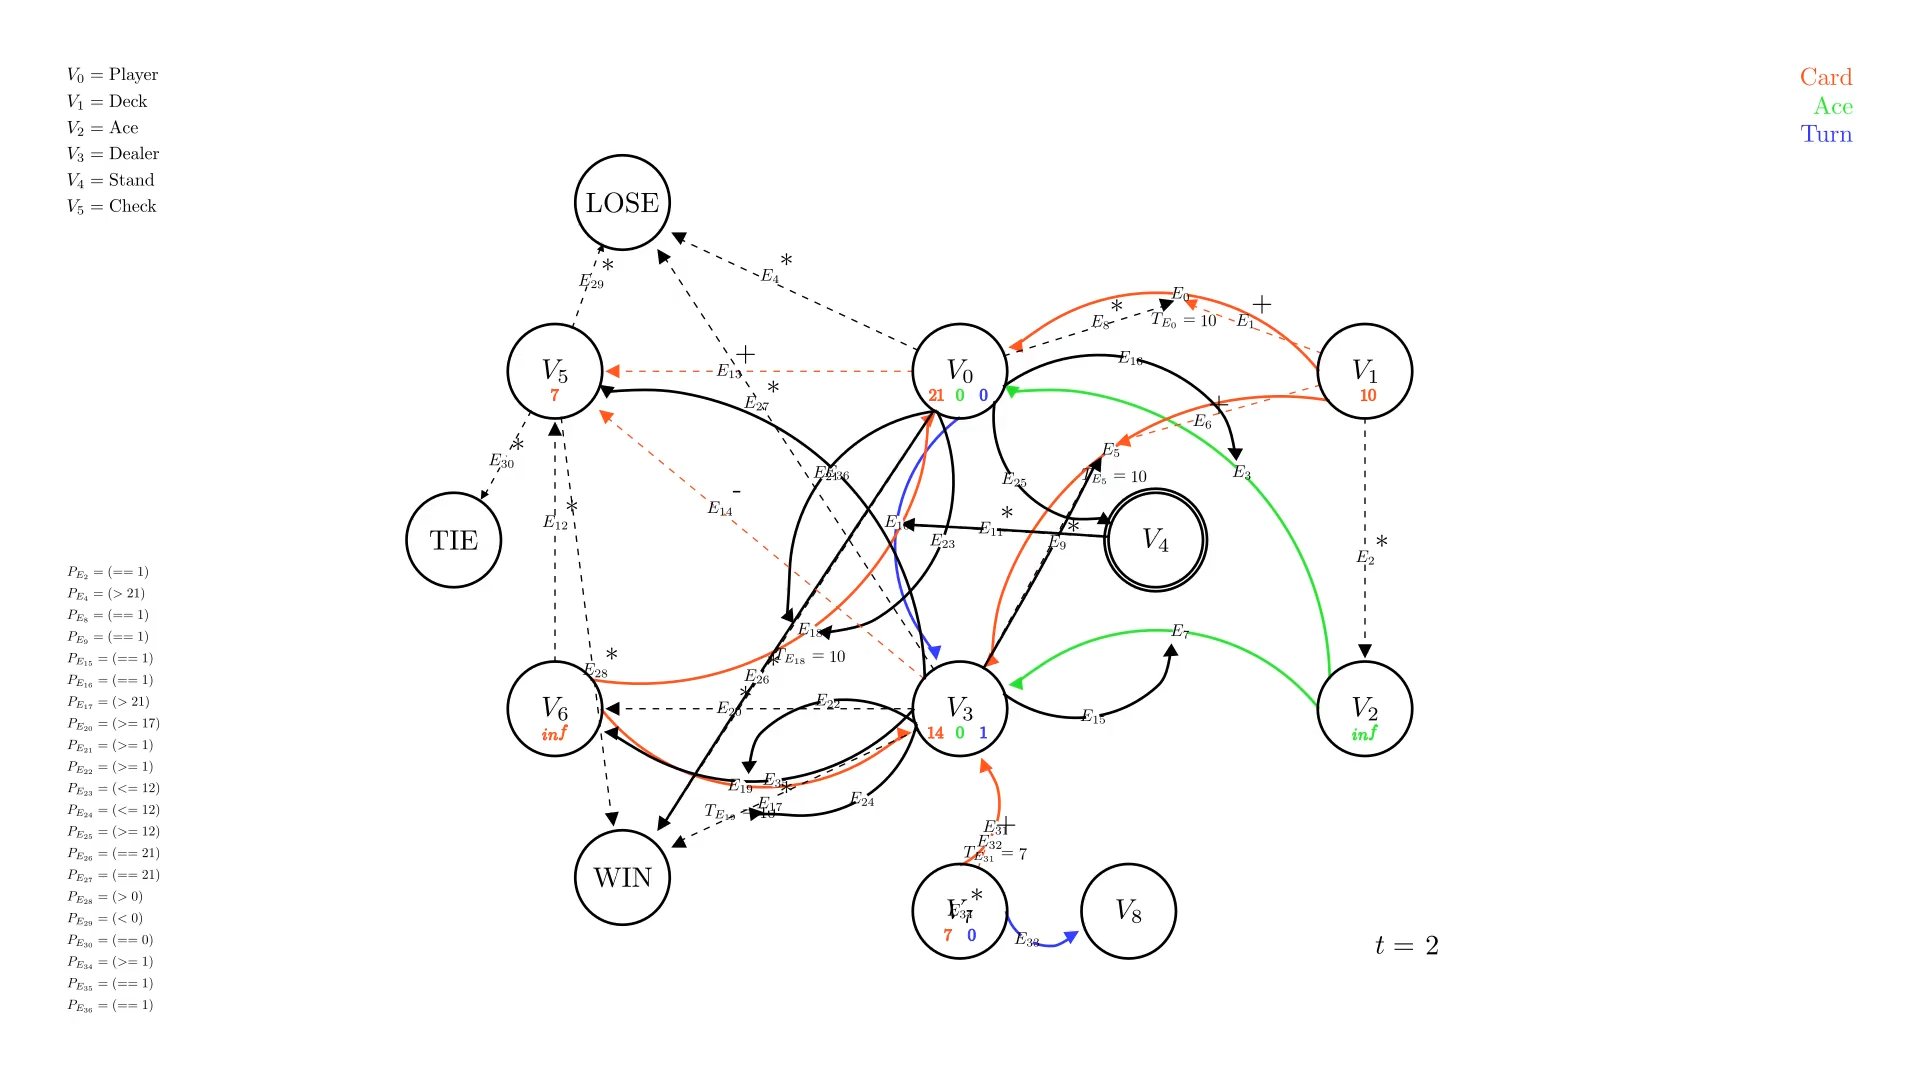
\includegraphics[width=1.2\linewidth]{figures/Blackjack.png}
    \caption{Representação do jogo \textit{Blackjack} sob a sintaxe implementada.}
    \label{fig:blackjack}
\end{figure*}

Assim, para cada especificação de diagrama Machinations, pode-se definir também os critérios específicos de recompensa conforme cada um dos nós. Ainda, a definição da função de potencial $\Phi$ facilita a extensão do esquema de recompensas conforme novos critérios.

Adicionalmente, além de pesos para cada um dos elementos observáveis, o agente recebe uma recompensa de $+1$ ao atingir uma condição de vitória pré-estabelecida (representada pelo nó $\text{WIN}$), mas só recebe recompensas cujos pesos são negativos quando perde (ativando o nó $\text{LOSE}$), além da recompensa de $-1$.

\subsection{Jogos modelados}
A fim de verificar a aplicabilidade e coerência das regras aqui redefinidas, modelamos os jogos Blackjack e Monopoly -- sendo o último o jogo no qual vamos testar a aplicabilidade do aprendizado. Isso se deve ao fato do Monopoly ser o jogo mais explicitamente definido no trabalho de referência\cite{machinations}, ser facilmente representável e permitir expectativas claras com relação à política ótima.
\subsubsection{Blackjack}
A Figura \ref{fig:blackjack} ilustra uma representação do jogo Blackjack a partir das regras implementadas. Aqui, o jogador (representado pelo nó $V_0$) recebe cartas do baralho ($V_1$) amostradas pelo modo de ativação não-determinístico a todo instante $t$. Essa transferência só ocorre, entretanto, quando o jogador possui um recurso do tipo turno -- verificação representada pelo predicado $P_{E_8}$, representado na figura como $(= 1)$.

\begin{figure*}[h!]
    \centering
    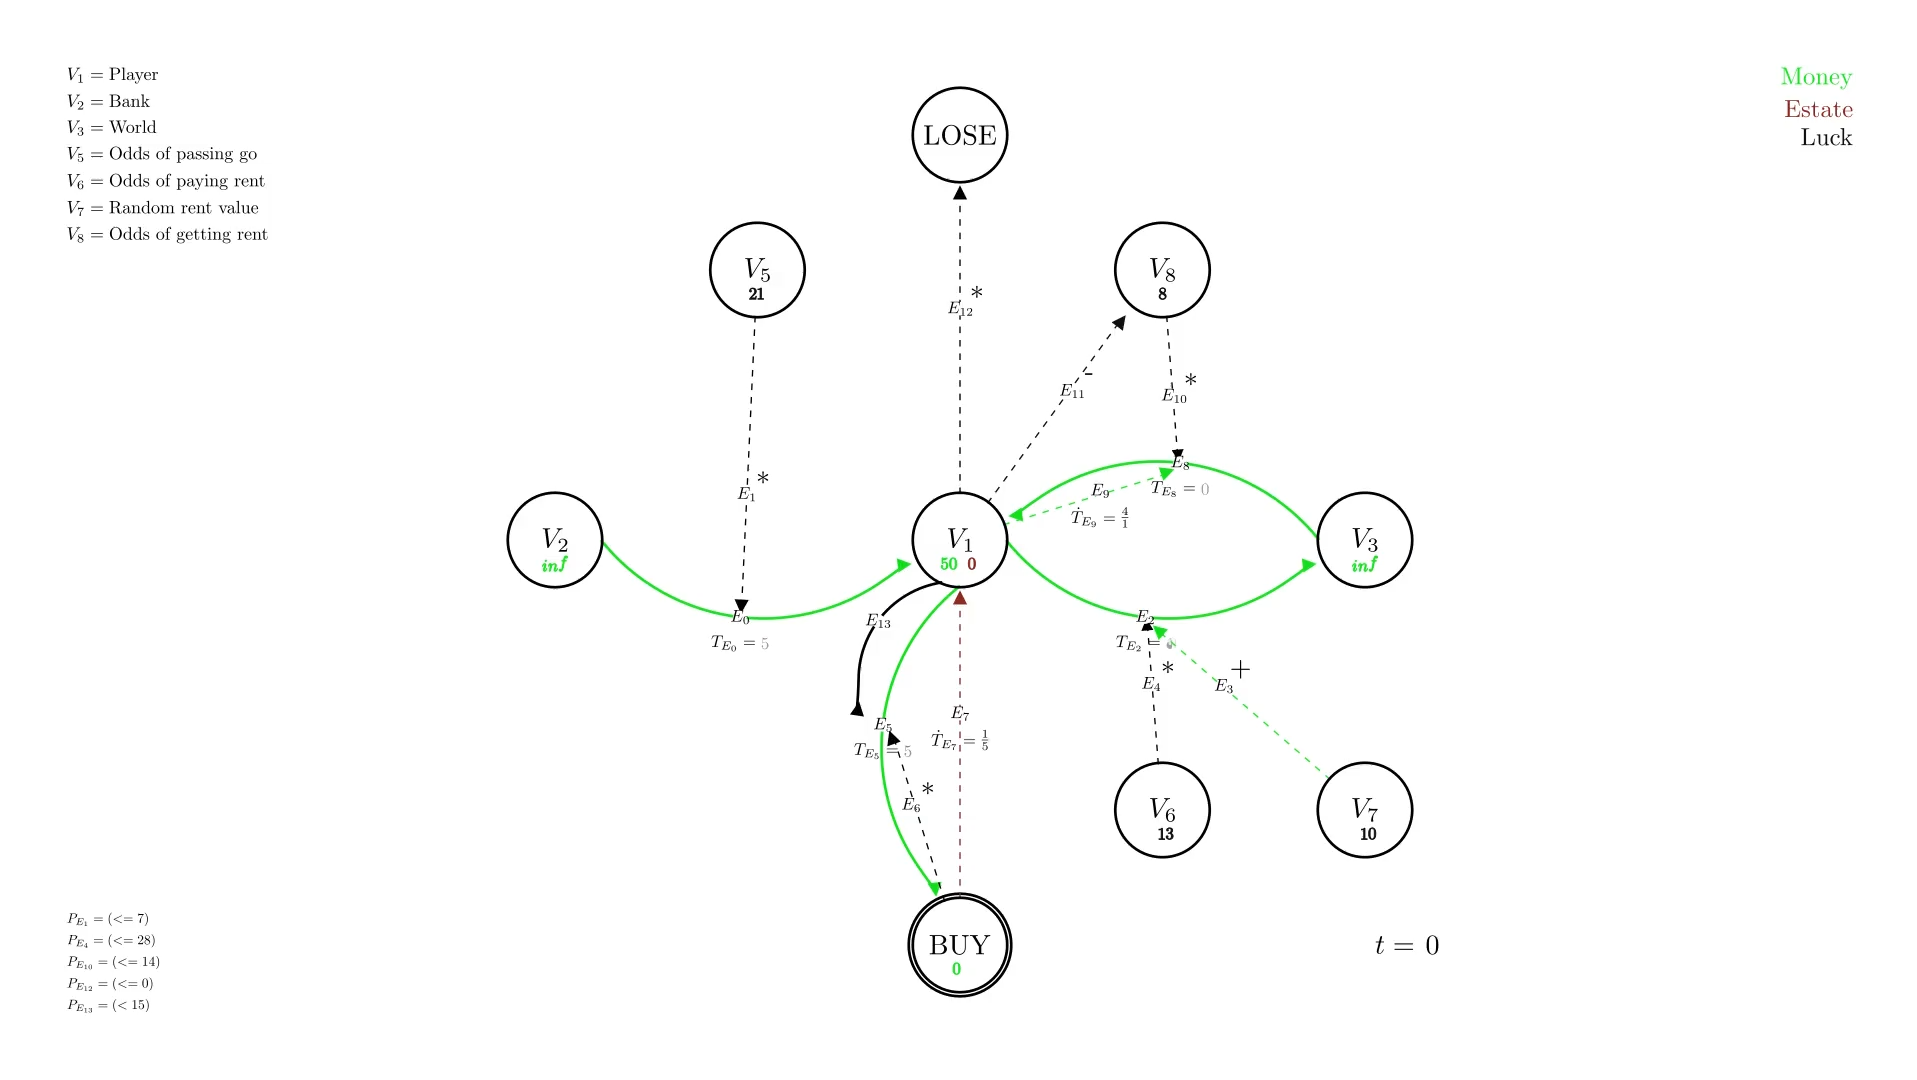
\includegraphics[width=1.2\linewidth]{figures/Monopoly.png}
    \caption{Representação do jogo \textit{Monopoly} sob a sintaxe implementada.}
    \label{fig:my-monopoly}
\end{figure*}

Ativar a ação $\text{STAND}$ ($V_4$) ativa, portanto, a transferência do único recurso turno do jogador para o dealer -- que, por uma lógica equivalente, recebe cartas do baralho a cada turno. O caso especial de cartas do tipo às, que contam 1 ou 11 no cenário de Blackjack conforme a vantagem do jogador ou dealer, é implementado pelo nó $V_2$. Sempre que o baralho ($V_1$) amostra uma carta, caso seu valor seja 1, $(P_{E_2})$, o gatilho $E_2$ ativa $V_2$, que tenta ativar as transferências $E_3$ e $E_7$ de um recurso do tipo "Ace" -- guardadas por ativadores que verificam se $V_0$ ou $V_3$ têm o turno.

O nó que verifica a condição de vitória ($V_6$) semelhantemente tenta transferir $10$ em valor de cartas para os nós $V_0$ e $V_3$ -- mas as conexões de recursos são guardadas por ativadores que verificam tanto a quantidade de cartas (um às não pode levar o jogador a mais que $21$) quanto a existência de um recurso do tipo "Ace". As saídas do jogo são representadas pelos nós especiais "WIN", "TIE" e "LOSE", que terminam o episódio com recompensas correspondentes quando ativados.

Observa-se que a representação de Blackjack a partir do conjunto de regras definidas é um tanto deselegante devido à intenção original que caracteriza a sintaxe Machinations: evidenciar comportamentos assintóticos ou padrões ao longo do tempo na economia de jogos. Sendo Blackjack um jogo com tipicamente menos de dez turnos, definidos por um conjunto de regras que é por si só mais simples que o diagrama construído, tentativas de aplicação de DQNs\cite{dqn} e PPO foram extremamente inefetivas na modelagem proposta e não serão elaboradas na Seção \ref{learning}.


\subsubsection{Monopoly}
\label{modeling:monopoly}
Ao simplificar o jogo Monopoly para aprendizado por reforço, visamos manter a representação do seu dilema central: o jogador deve investir para sobreviver a longo prazo, mas investir leva a uma posição vulnerável no curto prazo.

Assim, o jogador, representado pelo nó $V_1$, se vê em um ambiente onde é necessário tomar a ação "BUY" em algum momento para evitar a terminação do jogo por "LOSE" antes do limite de 30 turnos -- quando a recompensa positiva é dada. Para comprar uma propriedade (equivalente a comprar quadrados do tabuleiro), o jogador precisa transferir $\$5$ para o nó "BUY". Em seguida, o modificador de "BUY" para $V_1$ conta cada $\$5$ em "BUY" como uma propriedade em $V_1$. Aqui, evidenciamos a capacidade da sintaxe implementada de representar uma lógica recorrente em jogos: a troca de um recurso por outro.

A necessidade da compra de propriedades nesse cenário é dada pela mecânica de recebimento e pagamento de aluguel ao nó $V_3$, que representa (em uma abstração significativa) os demais jogadores. A cada turno, os nós $V_6$ e $V_8$ amostram valores aleatórios de $1$ a $40$ para seus estados, que são avaliados contra os predicados $P_{E_4} = (\leq 28)$ e $P_{E_{10}} = (\leq 14)$ para automaticamente ativar as conexões $E_2$ e $E_8$, respectivamente, com alguma chance a cada turno. O valor do aluguel pago pelo jogador via $E_2$ é determinado pelo valor aleatoriamente amostrado de $V_7$ dentre a distribuição $\{2, 4, 6, 10, 10, 12, 12, 15, 15\}$, abstraindo a variedade de eventos que podem causar transações negativas no saldo monetário do jogador.

A estratégia principal do jogo, por fim, é permitida pela ação dos modificadores $E_9$ e $E_{11}$, que aumentam a probabilidade de receber aluguel em $\frac{1}{40}$ e o valor recebido em $4$, respectivamente, para cada propriedade possuída por $V_1$. Adicionalmente, a mecânica do quadrado "GO" no mapa do jogo original é implementada por $V_2$, que, com probabilidade $\frac{7}{40}$, estimula a economia do jogo transferindo $\$5$ para o jogador.

Nesse cenário, como evidenciado na Seção \ref{results}, o $\Delta X_{V_1,R_0}$ (sendo $R_0$ o recurso que representa capital) esperado para cada turno dados os valores e probabilidades descritos é negativo -- em outras palavras, o agente se vê obrigado a decidir entre comprometer seu valor monetário e arriscar ir à falência por um aluguel muito alto no turno seguinte ou não comprar propriedades e ter uma alta probabilidade de ir à falência no longo prazo.

Esse cenário providencia um MDP altamente estocástico e um problema com claro comportamento ótimo (comprar o máximo de propriedades mantendo uma reserva segura de capital e agir conservadoramente daí para frente). Temos, assim, um exemplo suficientemente representativo das regras aqui descritas e implementadas para a validação contra técnicas de aprendizado por reforço.

\subsection{Aprendizado}
\label{learning}
Definimos o problema de aprendizado na simulação de Monopoly definida como sobreviver até o instante $t=30$ em um ambiente que naturalmente leva o agente à falência. O perfil do ambiente apresentado é indiretamente ilustrado pelos resultados observados nas Figuras \ref{fig:ep_lens_control_0} e \ref{fig:ep_lens_control_0}. Para aprendizado por reforço, é essencial analisar as características mais proeminentes do ambiente: especificamente, trabalhamos com episódios curtos, recompensas somente no fim do episódio e um ambiente altamente estocástico. Isto significa que ações do agente e, portanto, alterações na política, não têm consequências imediatamente evidentes no espaço de observação.

A primeira tentativa de aprendizado foi feita com DQNs\cite{dqn}. Mesmo com diferentes configurações de pesos de recompensa e hiperparâmetros, essa solução não foi capaz de convergir para uma política sequer aceitável no ambiente apresentado. Atribuímos esses resultados à dificuldade da estratégia central de Q-Learning, mesmo dadas as soluções adicionais em DQNs, perante um ambiente com alta variância, dificultando a avaliação correta das ações. Além disso, a presença de recompensas esparsas e dadas somente ao final providencia um sinal insuficiente para a otimização adequada, especialmente para a detecção de nuances para escapar de ótimos locais.

Minimizando a dependência de uma estimativa clara da função de valor, a estratégia de Proximal Policy Optimization\cite{ppo} é a alternativa mais promissora dados os obstáculos apresentados. Isso porque a adoção de Generalized Advantage Estimation possibilita a propagação de sinais de recompensa mais fracos (descontados e dados ao final do episódio) para que se tornem visíveis apesar do ruído introduzido pela estocasticidade. Além disso, o clipped-surrogate objective proposto por Schulman et al. (2017) permite um aprendizado um pouco mais estável comparado às DQNs por limitar atualizações drásticas à política.

A Tabela \ref{tab:ppo_hyperparams} lista os hiperparâmetros empiricamente encontrados que produzem os melhores resultados, descritos na seção seguinte.

\begin{table}[h!]
\caption{Hiperparâmetros utilizados na aplicação de PPO ao ambiente que simula o jogo Monopoly}
\begin{center}
\begin{tabular}{|l|c|}
\hline
\textbf{Hiperparâmetro}              & \textbf{Valor}    \\
\hline
Taxa de aprendizado                  & $5\times10^{-4}$  \\
\hline
Fator de desconto                    & $0.98$            \\
\hline
Suavização GAE                       & $0.95$            \\
\hline
Comprimento do rollout               & $4096$            \\
\hline
Tamanho do batch                     & $128$             \\
\hline
Épocas por atualização               & $15$              \\
\hline
Intervalo de clipping                & $0.3$             \\
\hline
Coeficiente de entropia              & $0.05$            \\
\hline
Coeficiente de perda de valor        & $0.5$             \\
\hline
Norma máxima do gradiente            & $1.0$             \\
\hline
\end{tabular}
\label{tab:ppo_hyperparams}
\end{center}
\end{table}


\section{Resultados}
\label{results}
A amostragem de episódios produzidos pelos comportamentos de não-compra e compra aleatória com 50\% de chance revela o padrão esperado na construção do ambiente: o agente que nunca compra ações vive, em média, 10.5 episódios do máximo de 30 conforme ilustrado na Figura \ref{fig:ep_lens_control_0}. O agente de ação aleatória tem uma performance um pouco melhor, sobrevivendo em média 14 episódios (vide Figura \ref{fig:ep_lens_control}), e consegue em múltiplos casos sobreviver até o trigésimo episódio. 

Dados os valores esperados do ambiente definido na Subseção \ref{modeling:monopoly}, sobreviver até o episódio final é tipicamente um indicativo de que o agente comprou pelo menos alguma propriedade tal que a variação esperada no seu saldo total seja positiva ao longo do tempo. Nesse caso, isso quer dizer que o agente sobreviveria para sempre na simulação apresentada.

\begin{figure}[htpb]
    \centering
    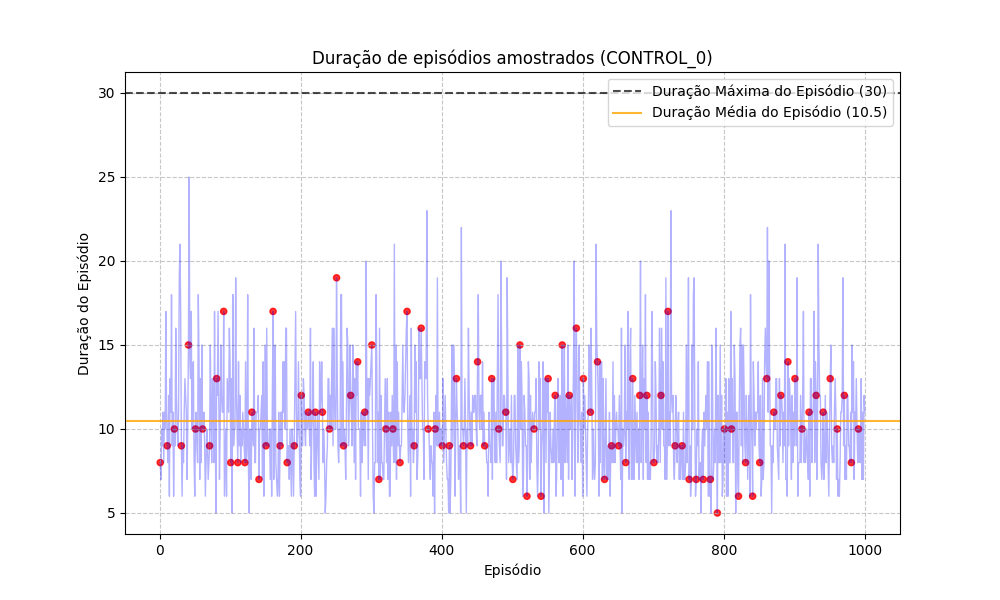
\includegraphics[width=1\linewidth]{figures/episode_lengths_control_0.png}
    \caption{Duração do episódio para 1000 episódios executados com um agente que nunca compra propriedades.}
    \label{fig:ep_lens_control_0}
\end{figure}

\begin{figure}[htpb]
    \centering
    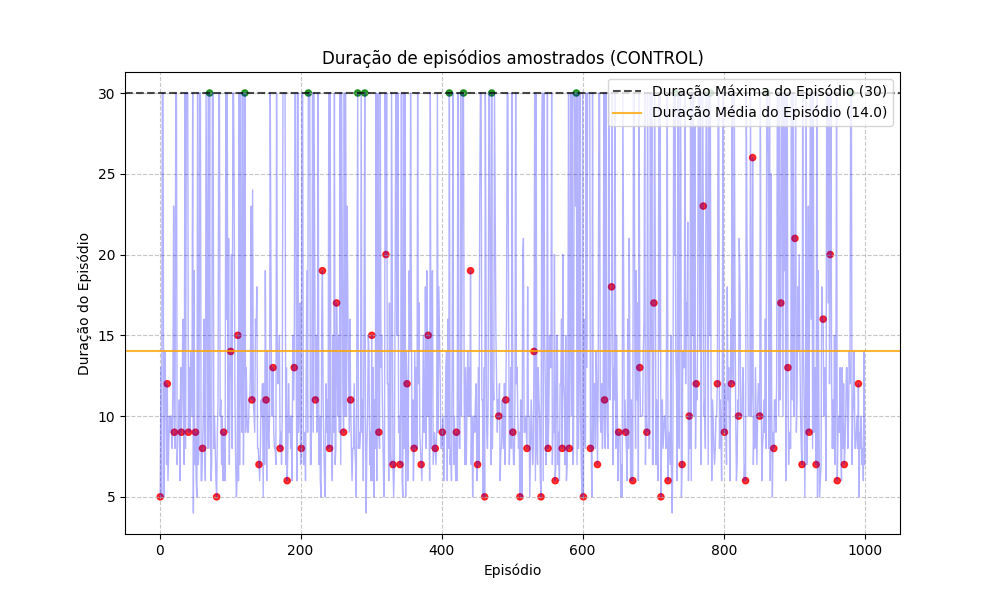
\includegraphics[width=1\linewidth]{figures/episode_lengths_control.png}
    \caption{Duração do episódio para 1000 episódios executados com um agente de escolha aleatória.}
    \label{fig:ep_lens_control}
\end{figure}

\begin{figure}[htpb]
    \centering
    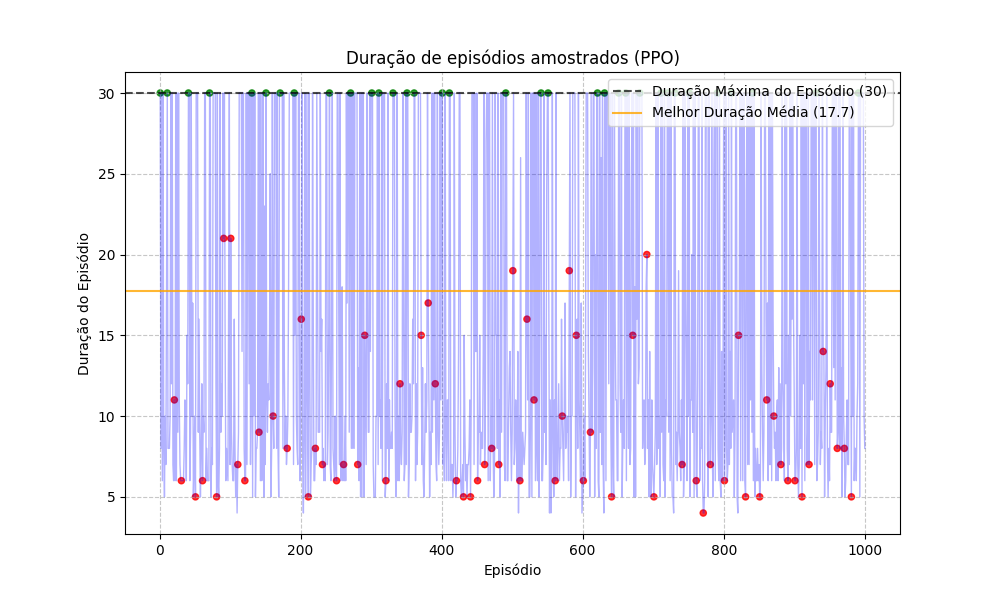
\includegraphics[width=1\linewidth]{figures/episode_lengths_ppo.png}
    \caption{Duração do episódio para 1000 episódios executados com um agente treinado por PPO durante 200.000 episódios.}
    \label{fig:ep_lens_ppo}
\end{figure}

\begin{figure}[htpb]
    \centering
    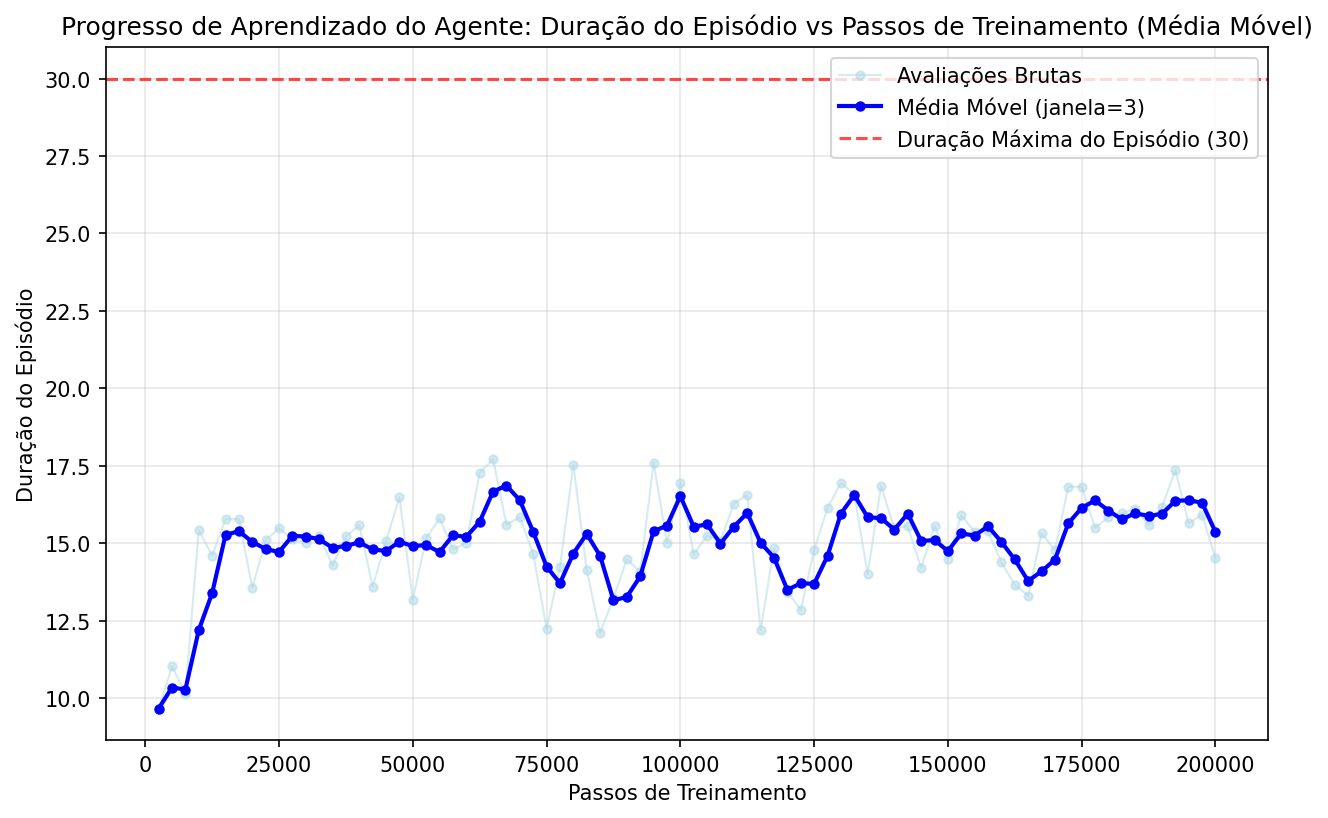
\includegraphics[width=1\linewidth]{figures/eval_progress.png}
    \caption{Progresso do treinamento do agente, medido pelo tempo de sobrevivência médio ao longo de 100 episódios de avaliação, executados a cada 2.500 etapas do treinmanto.}
    \label{fig:eval_progress}
\end{figure}

O agente obtido a partir do treino via PPO por 200.000 etapas considerando os hiperparâmetros na Tabela \ref{tab:ppo_hyperparams} performa levemente melhor que o agente aleatório, sobrevivendo uma média de 17.7 dos 30 episódios máximos e atingindo o episódio final mais frequentemente, conforme ilustrado pela Figura \ref{fig:ep_lens_ppo}. De fato, uma sobrevivência média de $+3.3$ turnos é suficiente para que o agente treinado por PPO vença frequentemente agentes aleatórios no cenário multijogador.

Observa-se a variância do ambiente pelas linhas azuis em todas as figuras dispostas nessa subseção -- além do ruído induzido pela estocasticidade, um padrão interessante se torna evidente: a frequência de "sucesso" de cada agente conforme os critérios definidos. Portanto, constatamos que o agente obtido supera a baseline aleatória, mas não é particularmente efetivo em capturar os padrões do ambiente. Especificamente, é comum que o agente ainda compre propriedades mesmo com baixo capital, levando a terminações prematuras mais frequentes que o caso ótimo.

Por meio dessa demonstração de caso, desde a construção do diagrama que representa um jogo até a aplicação efetiva de uma solução de aprendizado por reforço, validamos a hipótese de que é possível obter uma representação coerente às definições de um MDP e viável no quesito de aprendizado, mesmo quando altamente simplificada e estocástica. Entretanto, é necessário investigar a capacidade de transferência do caso simplificado para o caso geral, bem como planejar cuidadosamente a arquitetura e definições formais capazes de interceder os jogos modelados com suas implementações reais -- assim, a Seção \ref{future-work} define a direção dessa investigação como a segunda parte da presente Monografia em Sistemas de Informação.

\section{Considerações}

\subsection{Da qualidade das modelagens}
A construção de um conjunto de regras formais a partir da sintaxe proposta por Joris Dormans em Engineering Emergence é definitivamente a tarefa mais complexa e impactante para as demais etapas do trabalho. A busca por uma transcrição suportada pelo arcabouço de aprendizado por reforço mas ainda fiel ao trabalho original implicou em algumas concessões que significam que a sintaxe aqui implementada não é exatamente equivalente à do trabalho de referência. Esse é o caso para a maioria dos trabalhos na literatura de ciência da computação que visam implementar de maneira exata as definições um tanto descritivas da obra original\footnote{Vide \url{https://machinations.io/resources/academic-research-publications}}.

\subsection{Da estocasticidade dos ambientes}
A proposta de um diagrama Machinations é abstrair via relações lógicas e probabilidades comportamentos de um jogo definidos por um conjunto maior de regras mais complexas. Assim, o sinal recebido pelo agente, além de ser uma observação parcial do estado pela natureza dos jogos, é também parcial com relação à implementação completa do jogo. No caso do jogo Monopoly, por exemplo, abstrair todas as transações negativas para o jogador no pagamento periódico de aluguel não permite uma otimização convexa com relação às mecânicas originais que contemplam elementos como construções em cada quadrado do tabuleiro, o quadrado "JAIL", impostos, etc.

Entretanto, essa abstração naturalmente produz ambientes com sinais de gradiente mais ruidosos e de difícil identificação. Assim, somente as relações mais verdadeiramente explícitas são facilmente capturadas -- a depender do esquema de recompensas definido. Entretanto, relações sutis entre as features observadas e comportamentos mais complexos não têm espaço para se desenvolver em meio a um sinal de recompensa pouco evidente.

\section{Trabalhos futuros}
\label{future-work}
A direção natural para trabalhos futuros a partir da modelagem aqui definida é a tentativa de transferir o aprendizado advindo da simulação para o problema real no paradigma de curriculum learning\cite{curriculum}. Essa ideia induz, naturalmente, a hipótese de que a apresentação de diagramas cada vez mais complexos para o agente permite uma melhor aproximação para o problema -- que também merece investigação.

Ainda, é possível utilizar soluções model-based,  incluindo soluções mais tradicionais como Monte Carlo com aproximação de funções, para problemas curtos e estocásticos como Blackjack e Monopoly. Supõe-se que seja possível inferir uma função de transição aprimorada com comparação a um início aleatório, onde a complexidade do ambiente verdadeiro pode dificultar a identificação dos componentes-chave -- nesse caso, a modelagem cumpriria o papel de uma fase de "exploring starts" direcionada.

\vfill
\small O código implementado, as animações dos diagramas, os gráficos produzidos e os checkpoints dos modelos treinados estão disponíveis em \url{https://github.com/masganem/msi}. 
\newpage
\bibliographystyle{IEEEtran}
\bibliography{references}
\end{document}
